\begin{figure*}

  \begin{panel}{(a)}{\textwidth}
    \vspace{5mm}
    \small
    \tikzsetnextfilename{figure_1_overview}
    \usetikzlibrary{spy}%
\def\blinky#1#2#3#4#5{%
  \begin{tikzpicture}[node distance=3mm]
    \node[site#1] (s1) {};
    \node[site#2,right of=s1] (s2) {};
    \coordinate (s12) at ($(s1)!.5!(s2)$);
    \node[site#3,right of=s2] (s3) {};
    \node[site#4,below of=s12] (s4) {};
    \node[site#5,right of=s4] (s5) {};
    \foreach \angle in {0, 45, 90, 135, 180, 225, 270, 315}{
      \begin{scope}[rotate=\angle]
        \draw[sitelight#1] ($(s1)+(0,0.13)$) -- ($(s1)+(0,0.16)$);
        \draw[sitelight#2] ($(s2)+(0,0.13)$) -- ($(s2)+(0,0.16)$);
        \draw[sitelight#3] ($(s3)+(0,0.13)$) -- ($(s3)+(0,0.16)$);
        \draw[sitelight#4] ($(s4)+(0,0.13)$) -- ($(s4)+(0,0.16)$);
        \draw[sitelight#5] ($(s5)+(0,0.13)$) -- ($(s5)+(0,0.16)$);
      \end{scope}
    }
  \end{tikzpicture}
}%
\begin{tikzpicture}

  \begin{scope}[spy using outlines={magnification=2,size=12mm,very thick}]

    \node[image] (frame) {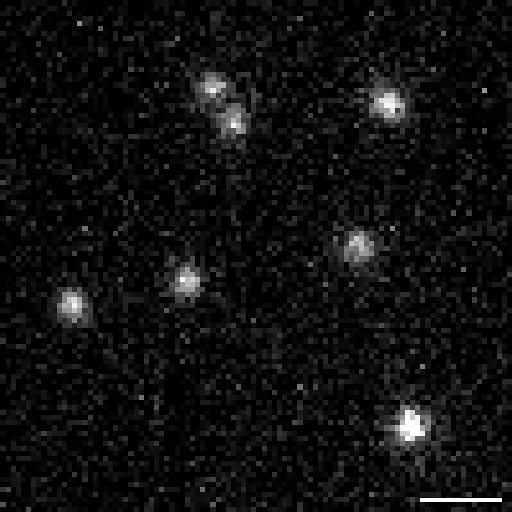
\includegraphics[width=4cm]{figures/data/overview/sample_frame}};

    \spy on ($(frame)+(1.1, 1.2)$)
      in node (patch_3) [image,right=6mm,anchor=north west]
      at (frame.north east);
    \spy on ($(frame)+(0.9, 1.1)$)
      in node (patch_2) [image,right=6mm,anchor=north west]
      at ($(frame.north east)-(0.1,0.1)$);
    \spy[
        draw=funkey_color_1,
        every spy on node/.append style={ultra thick},
        every spy in node/.append style={ultra thick},
        spy connection path={\draw[ultra thick] (tikzspyonnode) -- (tikzspyinnode);}
    ]
      on ($(frame)+(1.0, 1.2)$)
      in node (patch_1) [image,right=6mm,anchor=north west]
      at ($(frame.north east)-(0.2,0.2)$);
  \end{scope}

  % example trace
  \node[right=4mm,anchor=north west,text width=6cm,inner sep=0] (trace) at (patch_3.north east) {%
    \def\tracecsv{figures/data/overview/trace.csv}%
    \def\traceintensitycol{trace}%
    \def\nolabels{}%
    \tikzexternaldisable%
    \centerline{\begin{tikzpicture}%
  \begin{axis}[
    name=trace,
    width=0.8\textwidth,
    height=5cm,
    xlabel=frames,
    ylabel=intensity,
    enlarge x limits=false,
    xtick distance=500,
    grid=major,
    grid style={dashed},
    scaled ticks=false,
    ticklabel style={font=\small},
    legend style={nodes={scale=0.6, transform shape}},
  ]

    \addplot [
      color=tracecolor,
      mark=*,
      mark size=0.7pt,
      mark options={line width=0},
      fill opacity=0.8,
      draw opacity=0.2,
    ] table [
      col sep=comma,
      x=frames,
      y=\traceintensitycol
    ] {\tracecsv};
    \addlegendentry{intensity trace}

    \addplot [
      color=ztracecolor,
      thick
    ] table [
      col sep=comma,
      x=frames,
      y=\zcol
    ] {\tracecsv};
    \addlegendentry{inferred state}

    % remember min/max y-axis values for next plot
    \pgfplotsextra{
      \pgfmathparse{\pgfkeysvalueof{/pgfplots/ymin}}
      \global\let\ymin\pgfmathresult
      \pgfmathparse{\pgfkeysvalueof{/pgfplots/ymax}}
      \global\let\ymax\pgfmathresult
    }

  \end{axis}

  \begin{axis}[
    at={($(trace.east) + (4mm,0)$)},
    anchor=west,
    width=0.3\textwidth,
    height=5cm,
    yticklabel=\empty,
    xtick distance=0.005,
    xlabel=probability,
    grid=major,
    grid style={dashed, very thin},
    enlarge x limits={value=0.1,upper},
    scaled ticks=false,
    ymin=\ymin,
    ymax=\ymax,
    ticklabel style={font=\small},
    legend style={nodes={scale=0.6, transform shape}},
  ]

    \addplot+[
      xbar interval,
      mark=none,
      color=tracecolor,
      fill=tracecolor,
      fill opacity=0.6,
      draw=none,
    ] table [
      col sep=comma,
      y=\histbincol,
      x=\histcountcol,
    ] {\histogramcsv};
    \addlegendentry{intensity histogram}

    \addplot[
      color=intensitymodelcolor!80!black,
      thick
    ] table [
      col sep=comma,
      y=\histbincol,
      x=\modelfitcol
    ] {\histogramcsv};
    \addlegendentry{inferred model}

  \end{axis}
\end{tikzpicture}%
}%
    \tikzexternalenable%
  };
  \node[anchor=north,inner sep=0pt] at (trace.230) {\tiny time};
  \node[rotate=90,anchor=south,inner sep=1pt] at (trace.west) {\tiny intensity};

  % observed / hidden line
  \draw[gray,very thick]
    (patch_1.west|-frame.355) --
      node[pos=0,anchor=south west] {observed}
      node[pos=0,anchor=north west] {hidden}
      node[pos=0.35] (sample_1) {}
      node[pos=0.60] (sample_2) {}
      node[pos=0.96] (sample_3) {}
    (trace.east|-frame.355);

  % brace to MLE
  \draw[decorate,decoration={brace,raise=2mm}]
    (trace.north east) --
    node[pos=0.5,right=5mm,draw,rectangle,rounded corners] (mle) {\ours}
    (trace.south east);

  % posterior
  \node[anchor=north west,text width=3.6cm] (posterior) at ($(trace.north east)+(1.8,0.3)$) {%
    \def\posteriorcsv{figures/data/overview/posterior.csv}%
    \def\posteriorcol{posterior}%
    \def\noylabels{}%
    \tikzexternaldisable%
    \@ifundefined{noylabels}{}{%
  \pgfplotsset{yticklabel=\empty}%
}%
\begin{tikzpicture}%

  \def\eps{0.001}

  \begin{axis}[
    width=\textwidth,
    height=\textwidth,
    xlabel=\n,
    xlabel=$p(\n|\trace)$,
    grid=major,
    grid style={dashed, very thin},
    enlarge x limits=0.1,
    enlarge y limits=0,
    ymin=0,
    ymax=1,
    scaled ticks=false,
    ticklabel style={font=\small},
  ]

    \addplot+[
      ybar,
      bar width=1,
      mark=none,
      fill=posteriorcolor,
      fill opacity=0.6,
      draw=posteriorcolor,
      y filter/.expression={
        y < \eps ? nan : y
      },
    ] table [
      col sep=comma,
      y=\posteriorcol,
      x=n,
    ] {\posteriorcsv};

    \ifdefined\posteriorcolextra
      \addplot+[
        ybar,
        bar width=1,
        mark=none,
        fill=posteriorcolor!60!black,
        fill opacity=0.6,
        draw=posteriorcolor,
        y filter/.expression={
          y < \eps ? nan : y
        },
      ] table [
        col sep=comma,
        y=\posteriorcolextra,
        x=n,
      ] {\posteriorcsv};
    \fi

  \end{axis}

\end{tikzpicture}
%
    \tikzexternalenable%
  };
  \draw[arrow,shorten >=-8] (mle) -- (mle-|posterior.west);

  % blinky things
  \node (hidden) at (frame.330-|patch_1) {\blinky{off}{off}{off}{off}{off}};
  \node (z_sample_1) at (frame.330-|sample_1) {\blinky{on}{off}{on}{on}{off}};
  \node (z_sample_2) at (frame.330-|sample_2) {\blinky{on}{off}{on}{off}{off}};
  \node (z_sample_3) at (frame.330-|sample_3) {\blinky{on}{off}{off}{off}{off}};

  \draw[arrow] (z_sample_1) -- +(0, 2.4);
  \draw[arrow] (z_sample_2) -- +(0, 2.05);
  \draw[arrow] (z_sample_3) -- +(0, 1.7);

  \node[anchor=north,inner sep=10pt] at (hidden) {\strut$\n=5$};
  \node[anchor=north,inner sep=10pt] at (z_sample_1) {\strut$\z{}=3$};
  \node[anchor=north,inner sep=10pt] at (z_sample_2) {\strut$\z{}=2$};
  \node[anchor=north,inner sep=10pt] at (z_sample_3) {\strut$\z{}=1$};

\end{tikzpicture}

    \vspace{-4mm}
  \end{panel}

  \begin{panel}{(b)}{0.6\textwidth}
    \begin{panel}{}{\textwidth}
      \small
      \tikzsetnextfilename{figure_1_p_on_off}
      \centerline{\begin{tikzpicture}
  \node[siteoff,inner sep=4pt] (off) {};
  \node[siteon,right=2cm of off,inner sep=4pt] (on) {};
  \foreach \angle in {0, 45, 90, 135, 180, 225, 270, 315}{
    \begin{scope}[rotate=\angle]
      \draw[sitelighton,ultra thick] ($(on)+(0,0.26)$) -- ($(on)+(0,0.32)$);
    \end{scope}
  }
  \draw[arrow,shorten >=2mm,shorten <=2mm] (off) to[bend left] node[pos=0.5,above] (pon) {\pon} (on);
  \draw[arrow,shorten >=2mm,shorten <=2mm] (on) to[bend left] node[pos=0.5,below] {\poff} (off);

  \node[right=14mm of on] (re) {$\sim\poisson(\re\deltat)$};
  \draw[arrow,decorate,decoration={coil,aspect=0,segment length=6,post=curveto,post length=2mm}] ($(on.east)+(0.2,0)$) -- (re);

  %\node[parameters,anchor=south] at (re.north) {\strut$\parameterst = (\pon, \poff)$};

  \node[above=1mm of pon,gray] {transition model};
\end{tikzpicture}
}
    \end{panel}

    \vspace{4mm}
    \begin{panel}{(c)}{\textwidth}
      \small
      \hspace{4mm}
      \tikzsetnextfilename{figure_1_intensity_model}
      \begin{tikzpicture}

  \node (z) {\blinky{on}{off}{on}{on}{off}};
  \node[var,right=18mm of z] (c) {$\photons$};
  \node[annotation,below of=c] (c_dist) {$\sim\poisson((\z{}\re + \rb)\deltat)$};
  \draw (c) -- (c_dist);
  \draw[arrow,decorate,decoration={coil,aspect=0,segment length=6,post=curveto,post length=3mm}]
    (z.east) -- (c);

  \node[right=12mm of c,inner sep=0,yshift=2mm] (camera) {
    \tikz[plane x={(0.8,-0.4)},canvas is plane,transform shape]{
      \draw[gray,step=0.25] (0, 0) grid (1, 1);
      \node[anchor=south,gray] at (0.5, 1.1) {detector};
    }
  };

  \coordinate (camera_center) at (camera.center|-c);
  \draw[arrow,shorten >=3mm] (c) -- (camera_center);
  \node[observation,right=18mm of camera_center] (x) {$\x{}$};
  \node[annotation,below of=x] (x_dist) {$\sim\mathcal{N}(\photons\camgain + \camoffset, \camvar)$};
  \draw (x) -- (x_dist);
  \draw[arrow] (camera.east|-c) -- (x);
  \node[below=1mm of z] {\z{}};

  % parameter collections
  %\node[parameters,anchor=south west] at (z.north east) {\strut$\parameterse = (\re, \rb)$};
  %\node[parameters,anchor=south east] at (z.north-|x_dist.east) {\strut$\parametersc = (\camgain, \camoffset, \camvar)$};

  % annotations
  \node[above=2mm of c,gray] {\strut emission model};
  \node[above=2mm of x,gray] {\strut camera model};
\end{tikzpicture}

    \end{panel}
  \end{panel}
  \begin{panel}{(d)}{0.4\textwidth}
    \small
    \vspace{4mm}
    \hspace{4mm}
    \tikzsetnextfilename{figure_1_model}
    \centerline{\begin{tikzpicture}

  % parameters
  \node[var] (n) {\n};
  \node[var,below of=n] (theta_T) {\parameterst};
  \node[var,below of=theta_T] (theta_E) {\parameterse};
  \node[var,below of=theta_E] (theta_C) {\parametersc};

  % hidden states
  \node[state,right=1cm] (z1) at ($(n)!.5!(theta_T)$) {\z{1}};
  \node[state,right=4mm of z1] (z2) {\z{2}};
  \node[state,right=1cm of z2] (zt) {\z{t}};
  \node at ($(z2)!.5!(zt)$) {$\cdots$};

  % observations
  \node[observation,right=1cm] (x1) at ($(theta_E)!.5!(theta_C)$) {\x{1}};
  \node[observation,right=4mm of x1] (x2) {\x{2}};
  \node[observation,right=1cm of x2] (xt) {\x{t}};
  \node at ($(x2)!.5!(xt)$) {$\cdots$};

  % plates
  \begin{pgfonlayer}{background}
    \node[plate,fit=(z1)(zt)] (hidden) {};
    \node[plate,fit=(x1)(xt)] (observed) {};
  \end{pgfonlayer}

  % dependencies
  \draw[arrow] (n) to (hidden);
  \draw[arrow] (theta_T) to (hidden);
  \draw[arrow] (theta_E) to (observed);
  \draw[arrow] (theta_C) to (observed);
  \draw[arrow] (z1) to (x1);
  \draw[arrow] (z2) to (x2);
  \draw[arrow] (zt) to (xt);
  \draw[arrow] (z1) to (z2);
  \draw[arrow,shorten <=20] (z2) to (zt);
  \draw[shorten >=22] (z2) to (zt);

  % annotation
  \node[below of=observed] {$p(\trace|\n,\parameterst,\parameterse,\parametersc)$};

\end{tikzpicture}
}
  \end{panel}

  \caption{
      \panelref{a} Overview of the blinx method (scale bar: 1 $\mu$m)
      %
      \panelref{b} TODO
      %
      \panelref{c} TODO
      %
      \panelref{d} TODO \ours is based on a Hidden Markov Model who's
      parameters are optimized to build the final posterior distribution
  }
  \label{fig:method:overview}
\end{figure*}
